%*****************************************
\chapter{Future}\label{ch:future}
%*****************************************

\section{Panalogy Architecture}



\subsection{Recursive Loops and Infinite Recursive Tracing Descent}

If the focus on the tracing is controlled carefully, these potential
loops can be avoided.  How to detect and control these potential loops
is an interesting area of future automatic debugging research in
reflective control.

\subsection{Potential Future Uses for Low-Level Tracing}

Lower level objects maybe be interesting to focus on for research in
automatic abstraction and simulation of system components.  Optimizing
compilers could benefit from this area of future research.  E.g.
focusing on the CPU object could help to develop better run-time
register allocation models.

\subsection{Why Should You Use This Radically New Language?}

Because the language is very similar to Lisp, it has proven to be easy
for both expert and novice programmers to learn.  This has been my
experience with the four undergraduates that have worked within the
language, who learned it quickly, started writing their own macros to
facilitate their style, and one even made additions to the core
algorithms.

\section{Agent Speech Acts}

At any given point in time, each agent is pursuing a different variety
of goals.  Each agent executes actions in order to accomplish
collections of these goals.  We treat language communication as an
additional physical action that the agent can choose to perform in
order to accomplish its goals.

\section{Modelling Noise in Agent Communication}

\begin{figure}[bth]
  \center
  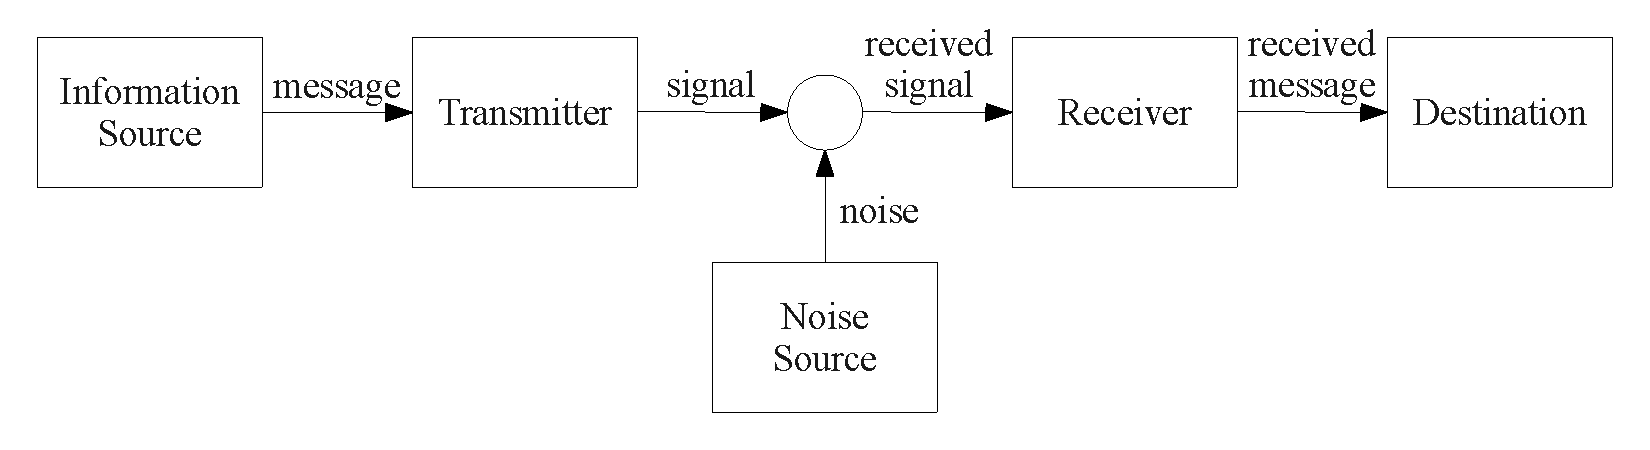
\includegraphics[width=10cm]{gfx/communication_theory}
  \caption[A mathematical theory of communication]{A mathamtical
    theory of communication~\citep{shannon:1959}.}
  \label{fig:communication_theory}
\end{figure}

Our cognitive theory makes no statements as to the presence of noise
in communication channels between agents and the environment.
Communication between agents and the environment in our implementation
occurs across a noiseless communication channel.  It is theoretically
possible to include a theory of noisy communication channels between
agents and the environment.  For example, Shannon's mathmematical
theory of communication~\citep{shannon:1959} could be applied as an
elaboration to any of the information pathways in our basic theory.


% horvat:
%
%   you consider the perception independent from the agent, i.e. many
%   agents can have the very same perception... against Schopenhauer:
%   "one can thus no longer separate the perceiver from the perception"
%   (The World as Will and Presentation) -> future work ;-)
%

\section{Applications to Education and Mental Health}

An exciting new field is growing to include applications of cognitive
theories of mind to both educational and clinical mental health
domains.  For example, \cite{mahncke:2006} have reported results of
improved cognitive function by using an automated computer cognitive
training program targeting age-related cognitive decline.

